\chapter{课题意义及国内外研究现状}

\section{引言}

现场可编程门阵列（FPGA）凭借可重构逻辑与灵活布线结构，已成为硅前验证的关键基础。基于FPGA的原型验证(FPGA Prototyping)通常能够以几十MHz的时钟频率运行，而传统软件RTL仿真器的仿真速度往往仅在千Hz（kHz）量级\cite{fujimoto_parallel_1990, nikolic_hardcloud_2019, chung_firesim_2018}。这意味着FPGA原型验证相较于软件仿真可实现数百倍甚至千倍以上的加速，使系统架构师能够验证完整软件栈并发现软硬件协同缺陷\cite{lattice_fpga_2013, kuon_measuring_2007}。然而，与软件仿真能够提供完整的可调波形不同，FPGA原型验证的可观测性长期受限，逻辑分析仪（Integrated Logic Analyzer）只能捕获预先选定的少数信号，难以支持大规模调试需求。

为解决信号可见性不足的问题，FPGA硬件仿真（FPGA Emulation）技术应运而生。其核心思想是在硬件运行过程中支持暂停、状态捕获与检查点（CheckPoint）导出，使工程师能够在不显著牺牲速度的前提下获取完整波形信息。这样既保留了原型验证的高运行速度，又显著增强了调试能力。

随着系统规模不断增加，单FPGA方案逐渐受到容量限制与编译时长的双重制约，难以满足现代片上系统（SoC）的验证需求。多FPGA系统因而成为主流选择。不论是原型验证系统异或是硬件仿真系统，构建多FPGA系统通常需要完成三个高度相关的关键步骤：划分（Partitioning）、集成（Integration）与互联（Interconnect）。

\paragraph{划分（Partitioning）}
大型设计需依据单FPGA的资源限制拆分为多个子设计。这会导致原始设计中的部分组合路径被切割成跨FPGA路径，使得相应信号必须通过额外的跨FPGA链路进行传输。划分质量直接决定跨FPGA数据量、系统性能以及后续步骤的复杂度。

\paragraph{集成（Integration）}
划分后的子设计无法直接运行在多FPGA硬件仿真体系中。为了支持暂停、恢复、检查点导出以及跨FPGA数据传输，需要在设计中插入多种辅助逻辑，包括扫描链、暂停控制逻辑、桥接与调度电路、跨FPGA信号的时序管理逻辑等。集成的目标是将子设计转化为可综合、可暂停、可观察、可重放的“硬件仿真就绪单元”，是原型验证系统与硬件仿真系统之间的关键差异所在。

\paragraph{互联（Interconnect）}
多FPGA系统需要通过高速互联结构将所有硬件节点连接在一起。互联不仅包括FPGA与FPGA之间的高速数据链路，也包括FPGA与主机之间的检查点传输和控制交互。此外，还需考虑物理链路（如LVDS、QSFP、PCIe）、流控机制、同步协议以及整体拓扑的可扩展性。互联结构直接影响系统性能、带宽平衡与扩展能力。

在工业界，HAPS、Palladium与Protium等商业加速与仿真平台已形成成熟体系，但其核心技术封闭、平台耦合度高，限制了可移植性。在学术界，已有FireAxe\cite{whangbo_fireaxe_2024}、Hetero-ViTAL\cite{zha_hetero-vital_2021}、DUOHUAFEN\cite{zhu_duohuafen_2024}与REMU\cite{chen_remu_2023}等开源尝试，其中FireAxe、Hetero-ViTAL与DUOHUAFEN主要面向多FPGA原型验证，而REMU聚焦单FPGA硬件仿真。迄今尚无完整的、可用的多FPGA硬件仿真系统。而且现有工作在划分策略、集成接口以及互联架构等方面仍存在显著限制，难以实现快速、灵活且可扩展的多FPGA硬件仿真部署。

在划分方面，现有系统如FireAxe仍需要用户手动参与，且依赖特定生态；Hetero-ViTAL 的Tile级划分粒度固定，灵活性有限；DUOHUAFEN基于超图的网表划分虽具潜力，但尚未支持更高层级的模块控制，缺乏一个开源、高度自动化且粒度可调的通用方案。

在集成方面，现有方法往往针对异步或特殊结构的多FPGA系统。例如，Hetero-ViTAL使用延迟不敏感（Latency-Insensitive， LI）技术，仅适用于握手解耦结构，无法支持组合逻辑切割；FireAxe的LI-BDN方法支持任意同步时序电路，但需要额外的组合依赖分析并引入复杂的握手控制；DUOHUAFEN的LI-TDM技术在轻量化和通用性方面更具优势。另一方面，REMU使用扫描链实现单FPGA硬件仿真，但无法直接适配划分后的多FPGA结构。因此，如何构建支持任意同步电路划分、适配多种互联结构并具备高效暂停与重放能力的集成方案仍是未解难题。

在互联方面，现有系统通常针对特定物理链路设计。如Hetero-ViTAL面向云平台采用以太网互联，延迟过高；FireAxe展示了多种链路方式，但缺乏统一的互联抽象；REMU基于PCIe与主机直连，但在多FPGA规模下难以扩展。目前仍缺乏一种能够屏蔽物理链路细节、支持异构拓扑并兼顾带宽、延迟与扩展性的互联框架。

综上，构建一个真正可用的多FPGA硬件仿真系统，需要在划分、集成和互联三个维度上提供更通用、更自动化且更可扩展的解决方案。

\section{背景知识与相关工作}

本节介绍该项目所使用的核心技术的背景知识以及项目的基础平台。首先，需要介绍超图与超图划分的概念，这是本项目实现通用RTL模块级划分的关键。然后介绍集成步骤中所使用的划分跨边界接口电路，从传统的延迟不敏感接口和分时复用接口，到DUOHUAFEN项目使用的LI-TDM。本项目的集成步骤将LI-TDM的控制状态机进行了修改以实现硬件仿真功能。最后，会介绍本项目所使用了两个基础平台：单FPGA硬件仿真平台REMU和多FPGA原型验证平台DUOHUAFEN。该项目将其融合，实现了多FPGA的硬件仿真平台。

\subsection{超图划分与电路划分}
电路划分技术的起源自电子设计自动化（EDA）的发展历程。早期研究致力于将网表划分以降低布局、布线和时序分析的复杂性，加快算法的执行效率\cite{kernighan_efficient_1970, breuer_class_1988, dunlop_procedure_1985}。在设计规模快速膨胀的今天，EDA的划分算法最小单元不再是标准单元库，而是模块。这能够在加快划分的求解速度的同时，保留了设计者的意图。

早期的网表划分方法通常采用图模型描述电路，运用最小割等启发式算法来最小化划分间的互连。然而随着电路复杂度提升，简单图模型已无法准确描述现代网表的多端口特性。\emph{超图}模型通过将边概念扩展为超边（可连接任意数量顶点）实现了更优的结构保真度\cite{alpert_recent_1995}。这种结构天然契合电路网络的建模需求：单个驱动器连接多个负载（超边），逻辑元件则作为顶点呈现。由此，电路划分任务被形式化为超图划分问题。其目标是在满足各分区资源分配平衡约束的前提下，最小化超边割集——即跨越多个分区的超边数量。这种抽象方式虽然适用于网表，但它忽略了节点之间或者超边之间的差异。如果想支持模块级划分的要求，还需要额外的扩展。

尽管近五十年的研究已催生出成熟的超图划分算法，但针对电路划分的开源工具仍存在显著应用缺口。工业领域主要依赖专有商业EDA工具：例如新思科技的ICC2虽采用先进的多级划分引擎，但其实现细节仍属保密。学术界虽存在众多通用的超图划分工具，但鲜有专门针对多FPGA的开源电路划分器设计。近期研究者开始将通用超图划分算法适配到电路网表划分这一领域，这凸显出开发可集成各类前沿超图划分算法的开源可扩展电路划分框架的重要性。TritonPart是一个电路划分领域的经典工作，尽管它不是面向FPGA原型验证，而是面向带有时序信息的网表\cite{tritonpart_2023}。但它支持的多约束驱动和多维权重是一个重要而通用的特性，恰好能满足了模块级划分的需求。另一方面，MaPart是一个面向FPGA原型验证的划分器，但是它不开源也不支持模块级划分\cite{li_mapart_2024}。

\subsection{划分跨边界接口电路}
管理跨FPGA边界数据交换是集成的重要目的之一，跨边界接口电路能够保证划分产生的中信号能够在正确进行跨FPGA的传递，从而实现多个子设计作为一个整体的功能正确性。在过去，主流的跨边界接口方法有延迟不敏感（Latency-Insensitive，LI）通信与分时复用（Time-Division Multiplexing，TDM）两种设计。

TDM和核心是串并转化，复用单个串行物理通道来传递多个并行的逻辑信号，从而解决I/O限制问题\cite{babb_virtual_1993}。为了能够在一个设计周期内传递多个信号的数据，TDM的一个设计周期内包含了多个信道传输的时钟周期。尽管它因为结构简单广泛被EDA公司采用，但这对系统时钟提出了极高的要求，TDM为了计算所有FPGA的系统时钟的周期和相位，要求物理信道具有确定性信号传播延迟，这种严格的时序约束使其不适用于通过PCIe或者网络互联的异步多FPGA平台，因这类平台会存在可变的传输延迟。

LI方法采用握手协议将模块内部时序与互连延迟解耦，将信号以数据包的形式在可靠的信道上传送。LI要求原始电路的I/O以寄存器为边界，并且时序电路可被暂停，以等待传送数据包造成的可变延迟，通常使用时钟门控或寄存器使能即可实现。虽然LI天然适用于使用FIFO解耦的模块化设计，但如果划分切口不是在寄存器边界，而是组合逻辑路径中间，LI就无法使用。为了解决组合逻辑的零延迟问题，延迟不敏感有界数据流网络（LI-BDN）被提出\cite{libdn_2009}。它通过为每个切口添加解耦的FIFO，能够正确的传递组合逻辑切口的中间信号。在此基础上，FireAxe通过添加组合依赖分析解决潜在的死锁问题，但这进一步增加了LI-BDN控制逻辑的复杂性\cite{whangbo_fireaxe_2024}。

DUOHUAFEN为了简化跨边界接口电路，实现通用性，设计了结合LI和TDM优点的LI-TDM的跨边界接口电路。首先，为了支持变化的物理信道延迟，LI-TDM对外的交互接口采用了延迟不敏感接口的设计思路。将跨节点传输信号跨边界接口为数据包，并使用可靠传输协议与互连组件交互，以保证数据包能够正确传递到对端。其次，为了支持组合逻辑的划分、简化控制逻辑，LI-TDM借鉴了TDM串并转换、复用一组物理连线的核心思想。LI-TDM通过打包和解包器，实现了复用同一套互联组件。不同的是，当跨片数据到达对端后，TDM由严格的时序约束控数据的采样时机，而LI-TDM则通过状态机记录所有组合电路完成运算后，再启动时序电路。这套跨边界接口电路既支持变化的物理信道延迟，又能适用于任意同步时序逻辑划分策略，且控制逻辑简单，资源占用少。因此，该项目拟采用LI-TDM作为划分的跨边界接口接口电路。

\subsection{多FPGA原型验证系统开发基础平台：DUOHUAFEN}

DUOHUAFEN是一个面向FPGA云上数字硬件逻辑设计的跨节点部署方案\cite{zhu_duohuafen_2024}。能够支持在不同层次的计算节点下，使用统一的流程和接口，部署数字设计的多FPGA的原型验证系统。为了实现通用性，DUOHUWFEN在“划分、集成、互联”三大关键步骤中均有关键的技术创新。

\begin{figure}[htb]
    \centering
    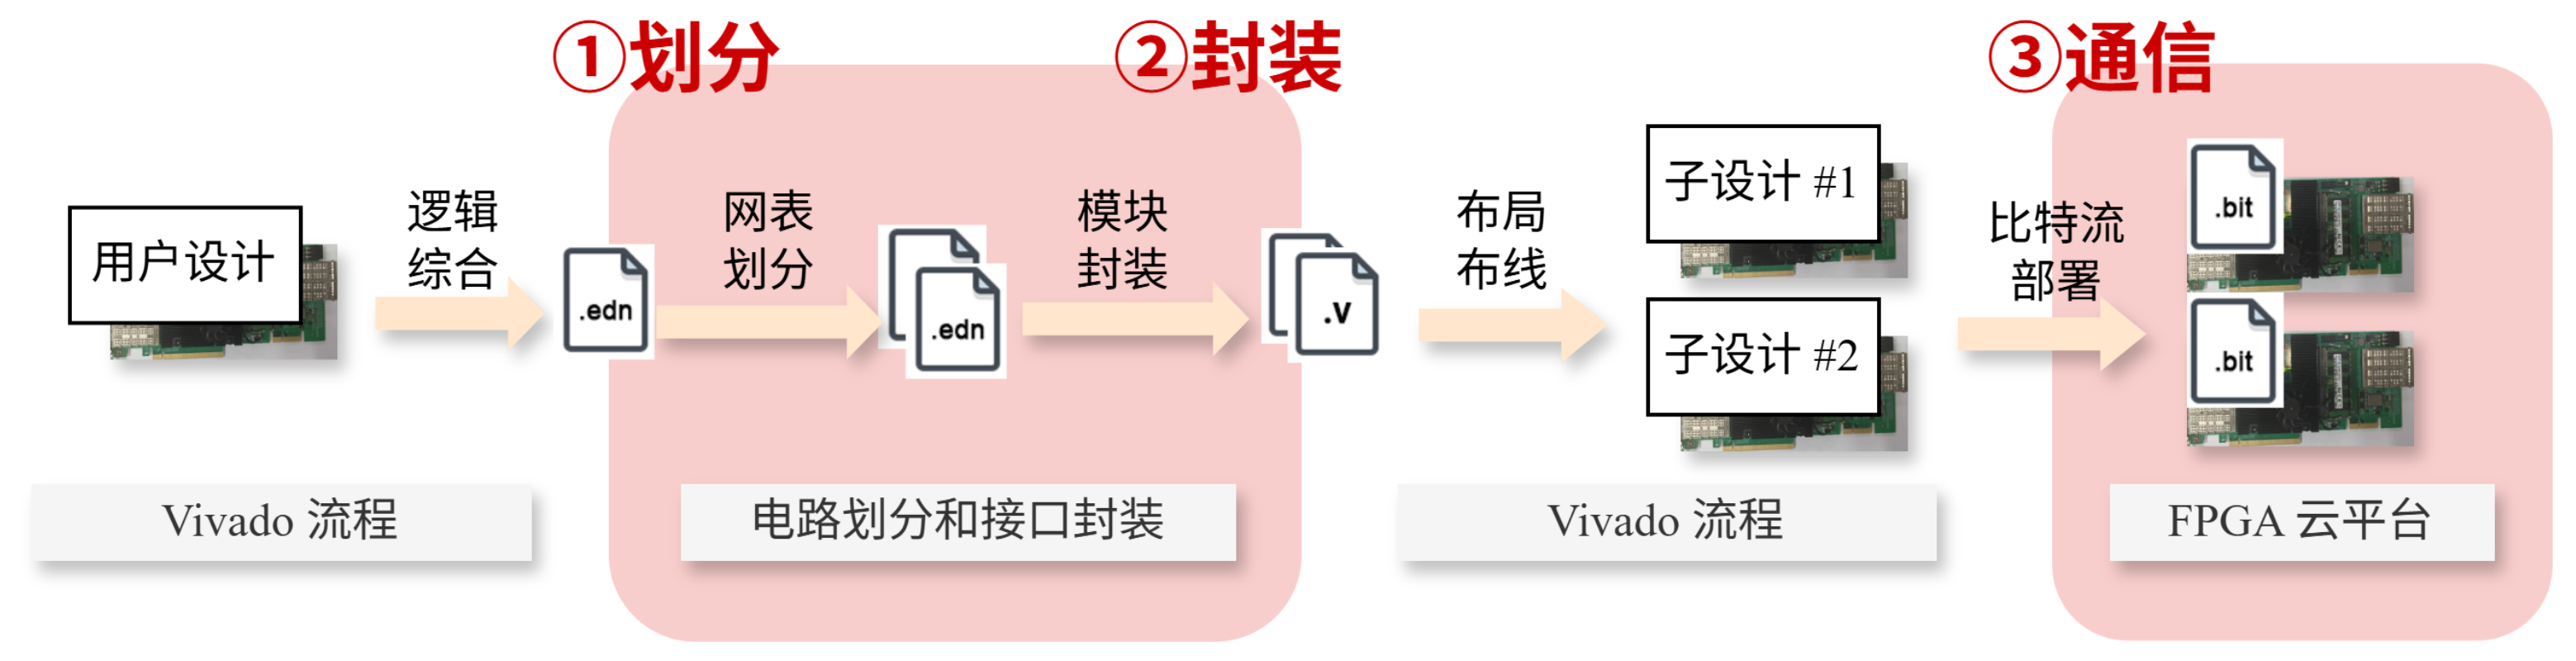
\includegraphics[width=\columnwidth]{figure/duohuafen-framework.png}
    \bicaption{DUOHUAFEN框架示意图}{DUOHUAFEN framework}
    \label{fig::duohuafen-framework}
\end{figure}

图\ref{fig::duohuafen-framework}展现了DUOHUAFEN的整体框架。在划分中，DUOHUAFEN实现了兼容标准EDIF网表格式与hMETIS超图格式的划分框架，能够将网表和超图进行双向转化，进而在电路划分领域集成了学术界典型的通用超图划分算法。本项目将延续集成超图划分算法的思路，进一步实现通用RTL的模块级划分和自适应粒度的划分。并将基于EDIF格式算法实现，进一步在广泛使用的综合器Yosys上实现。在集成中，DUOHUAFEN设计了结合LI和TDM优点的LI-TDM的跨边界接口电路。详见划分跨边界接口电路部分，在此不做赘述。在互联上，DUOHUAFEN提出了基于AXI-Stream协议的流式互连通信，用于为划分逻辑提供统一的跨节点数据交换接口，屏蔽了底层物理信道的差异。然后DUOHUAFEN依然是在同构的通信信道下构建多FPGA系统，本项目将在此基础上，利用物理信道无关的流失互联通信，在异构的通信信道中实现多FPGA的硬件仿真系统。


\subsection{硬件仿真系统开发基础平台：REMU}

REMU是一个周期精确、比特精确的FPGA硬件仿真平台\cite{chen_remu_2023}。图\ref{fig::remu-framework}展示了REMU平台的使用流程：用户仅需在主机上进行操作，通过基于PCIe的DMA数据通信，向FPGA发送控制信号。FPGA上运行着被插入扫描链的设计，设计可以被外部启动或者暂停，也可以将设计中所有时序器件的状态通过扫描链导入或导出。当x86主机获取状态检查点文件后，系统完整状态将被注入软件仿真器，在用户指定时段内实现电路级确定性重放。仿真过程中重建的波形文件包含被测设计所有电路级信号，为系统调试提供全比特精度可视化支持。

\begin{figure}[htb]
    \centering
    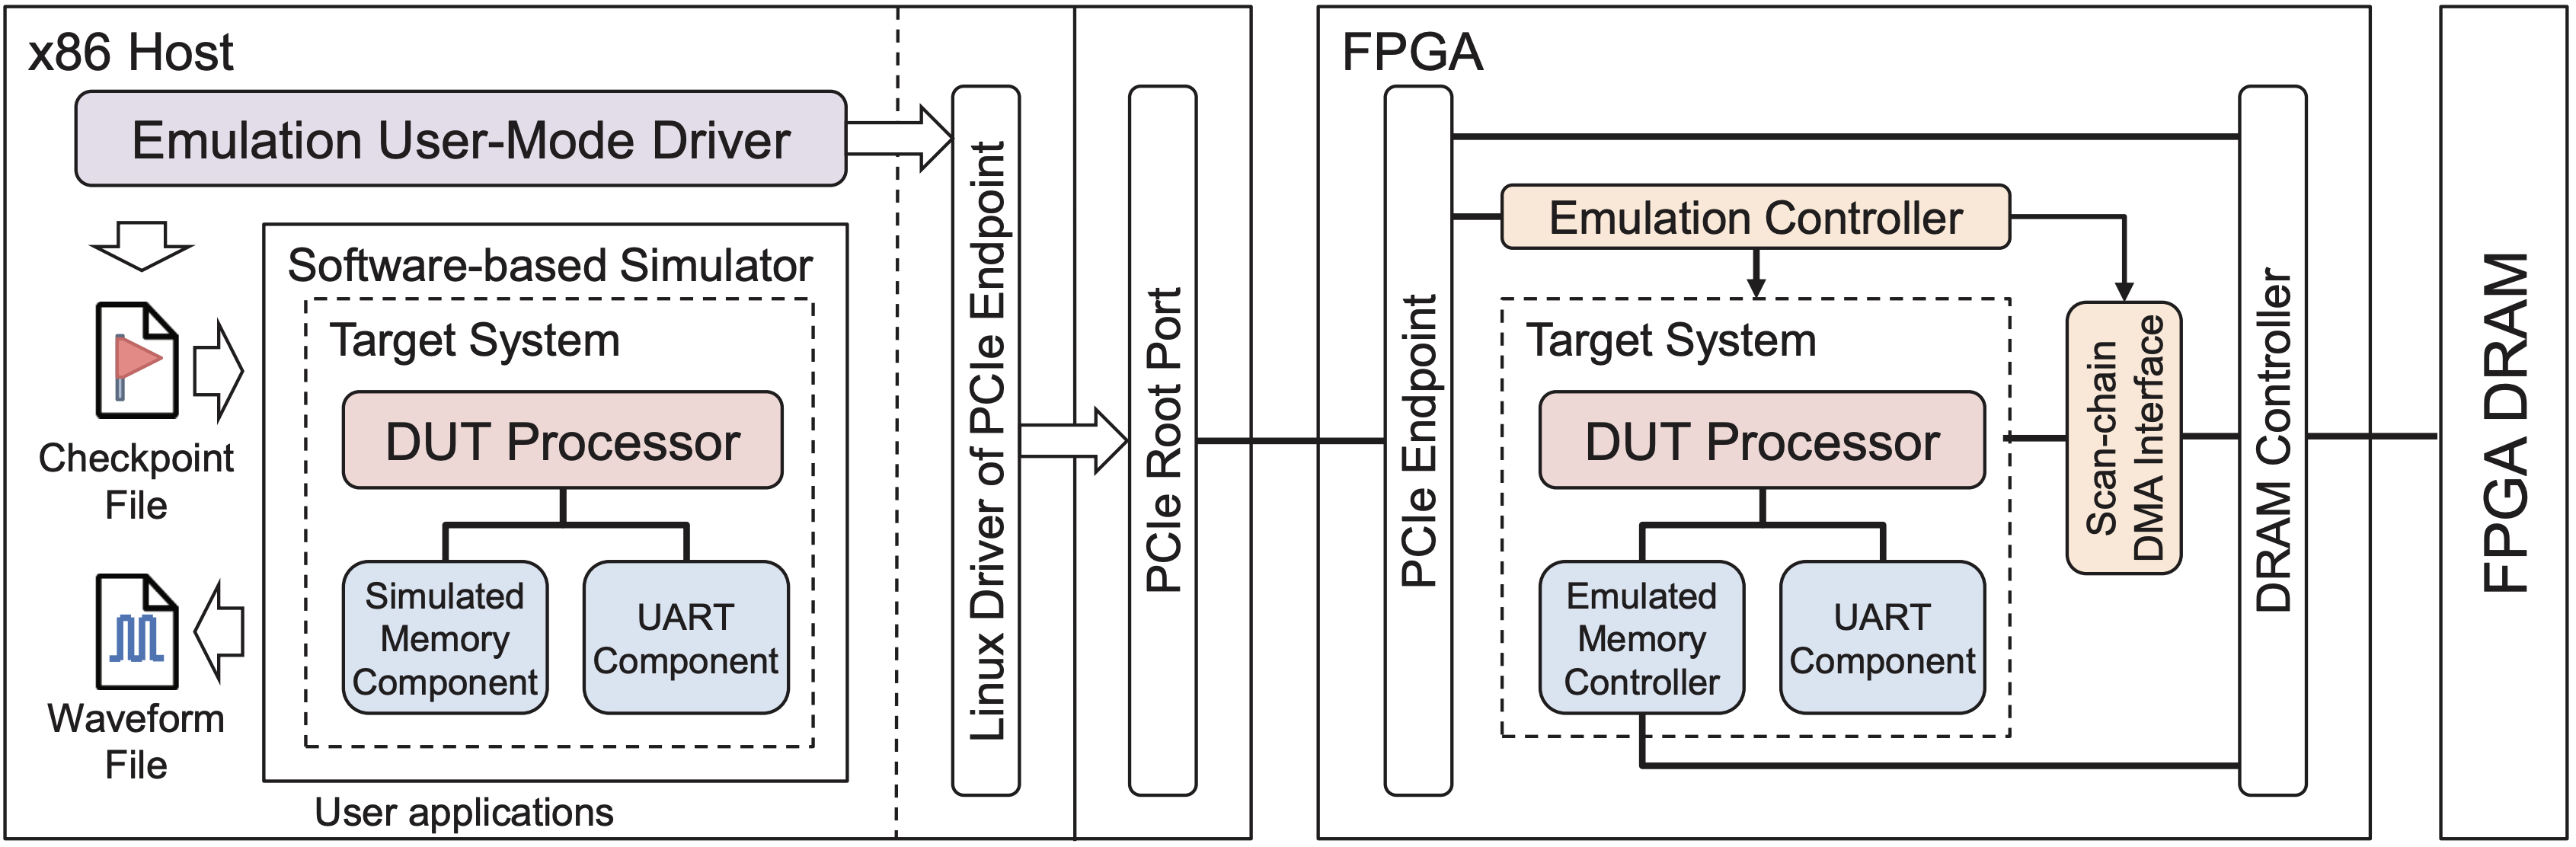
\includegraphics[width=\columnwidth]{figure/remu-framework.png}
    \bicaption{REMU硬件仿真系统整体框架}{REMU hardware emulation framework}
    \label{fig::remu-framework}
\end{figure}

为了实现全比特精确的波形重放，REMU使用了扫描链技术。扫描链的工作原理如图\ref{fig::scan-chain}所示，在开启扫描链模式的时候，时序器件的数据可以通过专用的数据通路导入或导出。相比未插入扫描链的设计，仅添加了额外的多路选择器、使能信号、以及扫描链数据通路，并未增加时序器件。扫描链是一种在不影响设计硬件电路功能的前提下，大大增加了信号可见性的方法。REMU编写了一套基于Yosys的自动化流程，用于处理时钟、插入扫描链、添加控制状态机。该课题将在原有框架下增加新的划分和集成的流程用于支持多FPGA的硬件仿真。

\begin{figure}[htb]
    \centering
    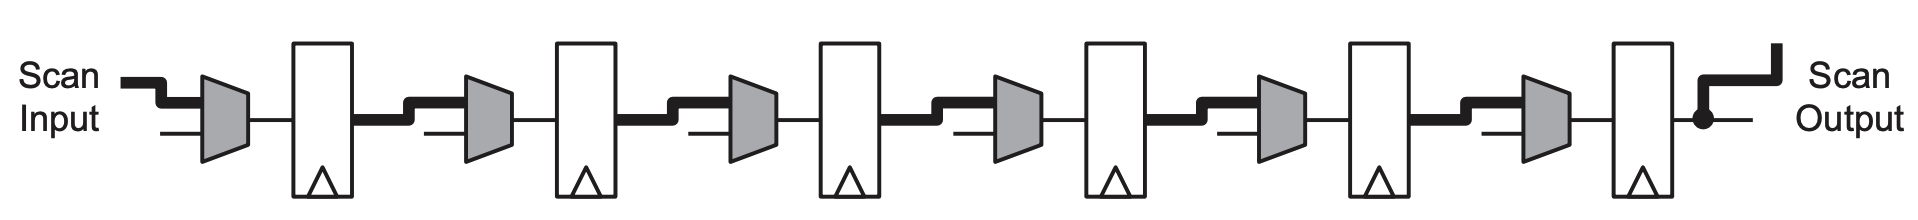
\includegraphics[width=\columnwidth]{figure/scan-chain.png}
    \bicaption{扫描链工作原理示意图}{Scan chain working principle}
    \label{fig::scan-chain}
\end{figure}

